\section{Taxonomy}
\label{sec:terminologies}

This section establishes a common framework, and defines common terminologies used throughout the
paper. We first describe a preprocessing step that turns a regular grid of values into a
\emph{stream} of \emph{chunks}, each of which slightly improves data's resolution or precision
(Section \ref{sec:raw-to-stream}). We then define the concepts of \emph{static} and \emph{dynamic}
streams (Section \ref{sec:static-dynamic-streams}), as well as discuss some of the most common
static streams (Section \ref{sec:common-static-streams}). Finally, we list all the data sets that are
used in experiments, with relevant properties (Section \ref{sec:data-sets}).

\subsection{Data streaming framework}
\label{sec:raw-to-stream}

Comparing different data reduction techniques is challenging. For example, it is difficult to force
a data subsampling method to use the same amount of data as a data quantization method for fair
comparison, because they reduce data in different sets of discrete steps. To tackle this problem, we
enforce one single step size which we call a \emph{chunk}.\pavol{maybe explain what chunk is here, but
I see the recursive definition issue} The data is first converted into a set of
\emph{chunks}, then the chunks can be ordered to form a \emph{stream} (\Cref{fig:pipeline}).

\begin{figure}[h]
  \centering
  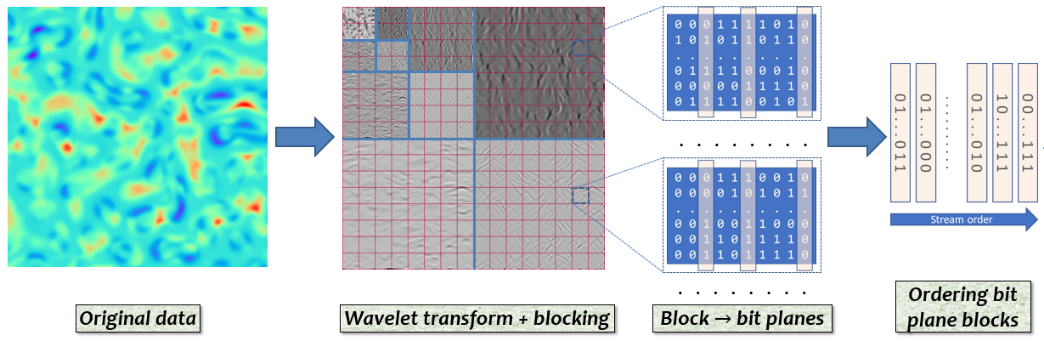
\includegraphics[width=\linewidth]{img/pipeline.png}
  \caption{Our data stream creation pipeline. The input is a regular grid of floating-point values,
  the output is a stream of chunks, where each chunk is a bit plane from a $4\times 4$ group of
  quantized wavelet coefficients, stored in negabinary format. The subbands are separated by blue
  lines in the second image, with the coarsest subband at the top left corner. TODO: revise this
  figure}
  \label{fig:pipeline}
\end{figure}


Different data reduction
techniques then can be represented with different ways of ordering chunks, or different streams.
To study the resolution-versus-precision tradeoffs in data analysis, however, we still need to
associate each chunk with a resolution and a precision level.

For resolution, we use the popular CDF5/3 discrete wavelet transform [CITE] to partition the data
into \emph{subbands}, each can be thought of as a resolution level. In the typical multi-dimensional
wavelet decomposition, one pass transform in 2D creates four subbands and in 3D eight subbands.. The first subband is a
smoothed, downsampled version of the original data. The next two subbands add fine details in each
dimension, respectively. The last subband adds fine details in both dimensions (or ``diagonal''
details) (see Figure \ref{fig:pipeline}). Subsequent transform pass iterates only on the first
subband created by the previous pass. We use $\bar{l}$ to denote the highest-numbered subband. In
this paper, $\bar{l}=9$ in 2D and $21$ in 3D, corresponding to three passes of transform.

For precision, we quantize the floating-point wavelet coefficients to $\bar{b}$-bit signed integers.
For most of the experiments in this paper, $\bar{b}=16$. This quantization eliminates the exponent
bits, so that every bit can be associated with a bit plane $b$ ($0\leq b\leq \bar{b}-1$). To further
avoid having to treat the sign bit specially in two's complement form, we convert the quantized
coefficients to negabinary form, in which integers are represented in base negative two (i.e.,
$v=\sum_{i=0}^{B}{c_i(-2)^i}$ with $c_i\in \{0,1\}$). This transformation increases the number of
bit planes by one to compensate for the absence of the sign bit.

As mentioned before, our fundamental unit of data for streaming is a \emph{chunk} of bits. A chunk
consists of bits that belong to the same bit plane, from a group of $4\times 4$ negabinary wavelet
coefficients in the same subband. Although each bit can be a chunk itself, we use a chunk size of
$16$ bits because in practice, for performance reasons, bits are never read and transmitted one by
one. This choice also significantly speeds up our experiments without meaningfully affecting the
results. By definition, each chunk can be associated with a subband $l$ ($0\leq l\leq \bar{l}$) and
a bit plane $b$ ($0\leq b\leq \bar{b}$). Different streams can thus be compared based on whether
they prioritize chunks belonging to finer subbands or chunks belonging to less significant bit
planes. The rest of the paper discusses different streams for various analysis tasks, and compare
them on this basis. We use the convention that higher subband is finer (so $l=0$ means the coarsest
subband), and higher bit plane is more precise (so $b=0$ is the most significant bit plane).

\subsection{Static and dynamic streams}
\label{sec:static-dynamic-streams}

In our data streaming model, there is a ``server'' which serves data and a ``client'' which receives
data from the server. While they can be on the same machine, the server has full knowledge of the
data, but the client does not. Thus, when the client receives a chunk, it might not know where the
chunk should be deposited. A common solution to this problem is to have both the client and the
server agree beforehand on a static ordering of chunks, regardless of the data. We use the term
\emph{static stream} to refer to streams using this solution. In constrast, a \emph{dynamic stream}
is one in which the client is assumed to ``magically'' know the positions of chunks without any
prior agreement with the server. In theory, dynamic streams perform better than static streams
because they can use actual chunk values, not just chunk positions, to better prioritize important
chunks. However, including positions also means that dynamic streams are ill-suited for implementations, because in
practice, the cost associated with sending position information likely outweights any potential
benefit gained from better prioritization of chunks. Despite that, dynamic streams are studied in
this paper because they can serve as a benchmark to evaluate the performance of their static
counterparts.

\subsection{Four static streams}
\label{sec:common-static-streams}

A stream can be viewed as a collection of chunks, sorted in descending order by weight
associated with each chunk $c$. In the literature, two of the most common orderings are \emph{by
level} and \emph{by bit plane}. The \emph{by level} stream orders the chunks strictly from coarser
to finer resolution levels. The weight function used by this stream is $W_1(c)=\bar{l}-L(c)$, where
$L$ is a function that returns the subband of a given chunk $c$ (with $0$ being the coarsest), and
$\bar{l}$ is the total number of subbands. Within the same subband, without any assumption on the
underlying data, the chunks naturally follow the row-major order. The other common ordering,
\emph{by bit plane}, proceeds strictly from higher-ordered to lower-ordered bit planes. That is,
$W_2(c)=\bar{b}-B(c)$, where $B$ is a function that map a chunk $c$ to the corresponding bit plane
and $\bar{b}$ is the total number of bit planes, with $0$ being the most significant.

The \emph{by level} and \emph{by bit plane} streams are designed to mimic the way data is progressively
accessed in traditional methods that work either in resolution (\emph{by level}) or in
precision (\emph{by bit plane}). We also define a third stream, called \emph{by
wavelet norm}, which combines these two dimensions. The \emph{by wavelet norm} stream orders chunks using
$W_3(c)=2^{\bar{b}-1-B(c)}\times \norm{\omega_{L(c)}}^2$. The term $2^{\bar{b}-1-B(c)}$ captures the
contribution of a bit on bit plane $B(c)$, while the term $\norm{\omega_{L(c)}}^2$ captures the
contribution of a coefficient on subband $L(c)$, where $\omega_{L(c)}$ refers to the wavelet basis
function on subband $L(c)$. The intuition behind \emph{by wavelet norm} is simply that in the
wavelet representation, a function $f$ is written as a linear sum of wavelet basis functions:
$f=\sum{c_i\omega_i}$, where $c_i$ are the coefficients and the basis functions $\omega_i$ in the
same subband have the same norm. Thus $W_3(c)$ is simply the contribution (in $L_2$ norm) of a bit
on bit plane $B(c)$ and subband $L(c)$ to the whole function $f$.

All the three streams mentioned so far are static. In addition, we also consider a
\emph{signature}-based stream to be static. A signature-based stream is one in which the server and
the client establish the agreement over chunk ordering through the transmission of a negligibly
small message, called signature, before any actual value bits are transmitted. A signature is a 2D
array with $\bar{l}$ rows and $\bar{b}$ columns, encoding the relative ordering of all possible
pairs $<l,b>$ for $0\leq l \leq \bar{l}$ and $0\leq b \leq \bar{b}$. We will show that the use of
such signatures can sometimes result in significant improvements over using purely static streams.
Section \ref{sec:stream-signature} gives a detailed discussion of the signature concept.

\subsection{Data sets}
\label{sec:data-sets}

Table~\ref{tbl:data-sets} contains all the data sets used for experiment in this paper. Note that
during pre-processing, all fields are converted to double-precision floating-point values before
quantization takes place. For ease of demonstration, as well as performance reason, the majority of
our experiments use 2D data sets. Often, these are slices from 3D volumes.
Section~\ref{sec:3d_results} presents our main results for 3D data sets. \pavol{we switched all to 3D right?}

\begin{table*}[t]
  \caption{Data sets used in experiments}
  \centering
  \begin{tabular}{p{0.15\linewidth}p{0.20\linewidth}p{0.15\linewidth}p{0.10\linewidth}p{0.15\linewidth}}
  \hline
  Name & Source & Slice dimension & Type & Citation\\
  \hline
  boiler & combustion simulation& $140\times 148$ & float64 &\\
  euler & fluid simulation& $256\times 1024$ & float64 &\\
  kingsnake & CT scan & $1024\times 795$ & uint8 &\\
  plasma & magnetic reconnection simulation& $512\times 512$ & float32 &\\
  marschner-lobb & analytical function& $256\times 256$ & float64 &\\
  diffusivity & hydrodynamics simulation& $384\times 384$ & float64 &\\
  pressure & hydrodynamics simulation& $384\times 384$ & float64 &\\
  velocityz & hydrodynamics simulation& $384\times 384$ & float64 &\\
  turbulence & fluid dynamics simulation& $256\times 256$ & float32 &\\
  \hline
  \end{tabular}
\label{tbl:data-sets}
\end{table*}
